\chapter{Attitude Determination Methods}\label{chap:EKF}

Attitude determination can be defined as finding the minimal parameterization of the attitude matrix whit the help of some measurement data. Generally speaking attitude determination methods can be divided into two categories. The first category are static methods. They relay only on measurements taken at the same time and are reliant on critical number of measurements at any given time to function. Examples of such methods are the TRIAD algorithm or solving Wahba's problem. The second category are filtering methods which uses a history of data and a dynamic model of the satellite. Examples of such models are variations of the Kalman filters \cite{SADCS}.        

\section{Attitude Determination Methods in CubeSats}
For attitude determination the extended Kalman filter (EKF) is the standard method and have a good record even if it has some problems. This problems mostly arises from the linearization that the filter performs \cite{attdetSur}. For the design of the MOVE-II attitude determination system (ADS) three other CubeSats ADS where studied \cite{DavidThesis}. 

\begin{itemize}
  \item \textbf{UWE3:} The third CubeSat of the University of Würzburg in Germany \cite{UWE-3}.
  \item \textbf{AAUSAT-3:} The third CubeSat of the Aalbord University in Denmark \cite{aausat}. 
  \item \textbf{ESTCube-1:} The first CubeSat of the University of Tartu, Estonia \cite{EST}.
\end{itemize}       

The ADS on all this systems have a lot of similarities to the ADS of MOVE-II. They are all based around the same sensors namely sun sensors, gyroscope and magnetometers. Because they have the same sensor set as the MOVE-II they also use many of the same models like the earth's magnetic field model and sun position model. In the end all this data is combined using some form of Kalman filter. They all vary slightly from each other and from the MOVE-II implementation. 

The UWE3 uses a Isotropic Kalman filter. The Isotropic Kalman filter is a recursive state estimation based on the dynamic model of the system. The state vector of the Kalman filter is the vector component of the quaternion and the bias of the gyroscope\cite{UWE-3}. The AAUSAT-3 uses a combination of an SVD-method to solve Wahba's problem and an unscented Kalman filter (UKF). Where the SVD-method is used to give a good initial estimate for the UKF. A UKF differs from a Kalman filter in that instead of using the last estimate to generate the prediction it uses a sigma point. Where a sigma point is a structured set of sampling points representing the probability distribution of the point. For a more in depth view look at \cite{attdetSur}. The ESTCube-1 also uses a UKF as their on board ADS. They also have a image-based attitude Simplified General Perturbationdetermination system that they use to verify the result of the UKF based ADS. The image-based system is done in a post processing proses on ground \cite{EST}

\section{Attitude Determination on MOVE-II}
The ADS on MOVE-II is based around an EKF that is initialized by the solution to Wahba's problem using SVD-methods. Overall structure of the ADS can be seen in \autoref{fig:ADS_overview}. There are two main parts going into the Attitude Determination Algorithms. The sensor measurements and the model output. The sensor measurements are preprocessed before they are sent to the algorithms. The models that are used will be future discussed in \autoref{subsec:ModelADS}. The SVD-method uses the model output and the sensor measurements to calculate an initial estimate for the EKF. The EKF then estimates the quaternion representing the rotation from Earth Centered Inertial frame (ECI) to the satellite body-fixed frame. The ECI is defined similarly to what is called the Geocentric Inertial Frame in \cite{SADCS}. Where the origin of the frame is at the center of mass of the earth. The z-axis is aligned with the earth's north pole. The x-axis is directed towards the vernal equinox. The vernal equinox the intersection of the earth's orbital plane and the earth's equatorial plane. The y-axis is defined to complete the coordinate frame with the right hand rule. The body-fixed frame is defined as having its origin at the center of mass of the satellite and the axis are parallel to the panels of the satellite. The z-axis is defined to point away from the top panel as shown in figure \autoref{fig:bodyFix}. The EKF also outputs an bias compensated angular velocity based on an estimate of the bias on the gyroscopes.

\begin{figure}[tbp]
	\centering
	\includegraphics[width=0.6\columnwidth]{./Pictures/GBF_new}
	\caption{The body-fixed frame drawn on the satellite from \cite{DavidThesis}}
	\label{fig:bodyFix}
\end{figure} 

\begin{figure}[tbp]
	\centering
	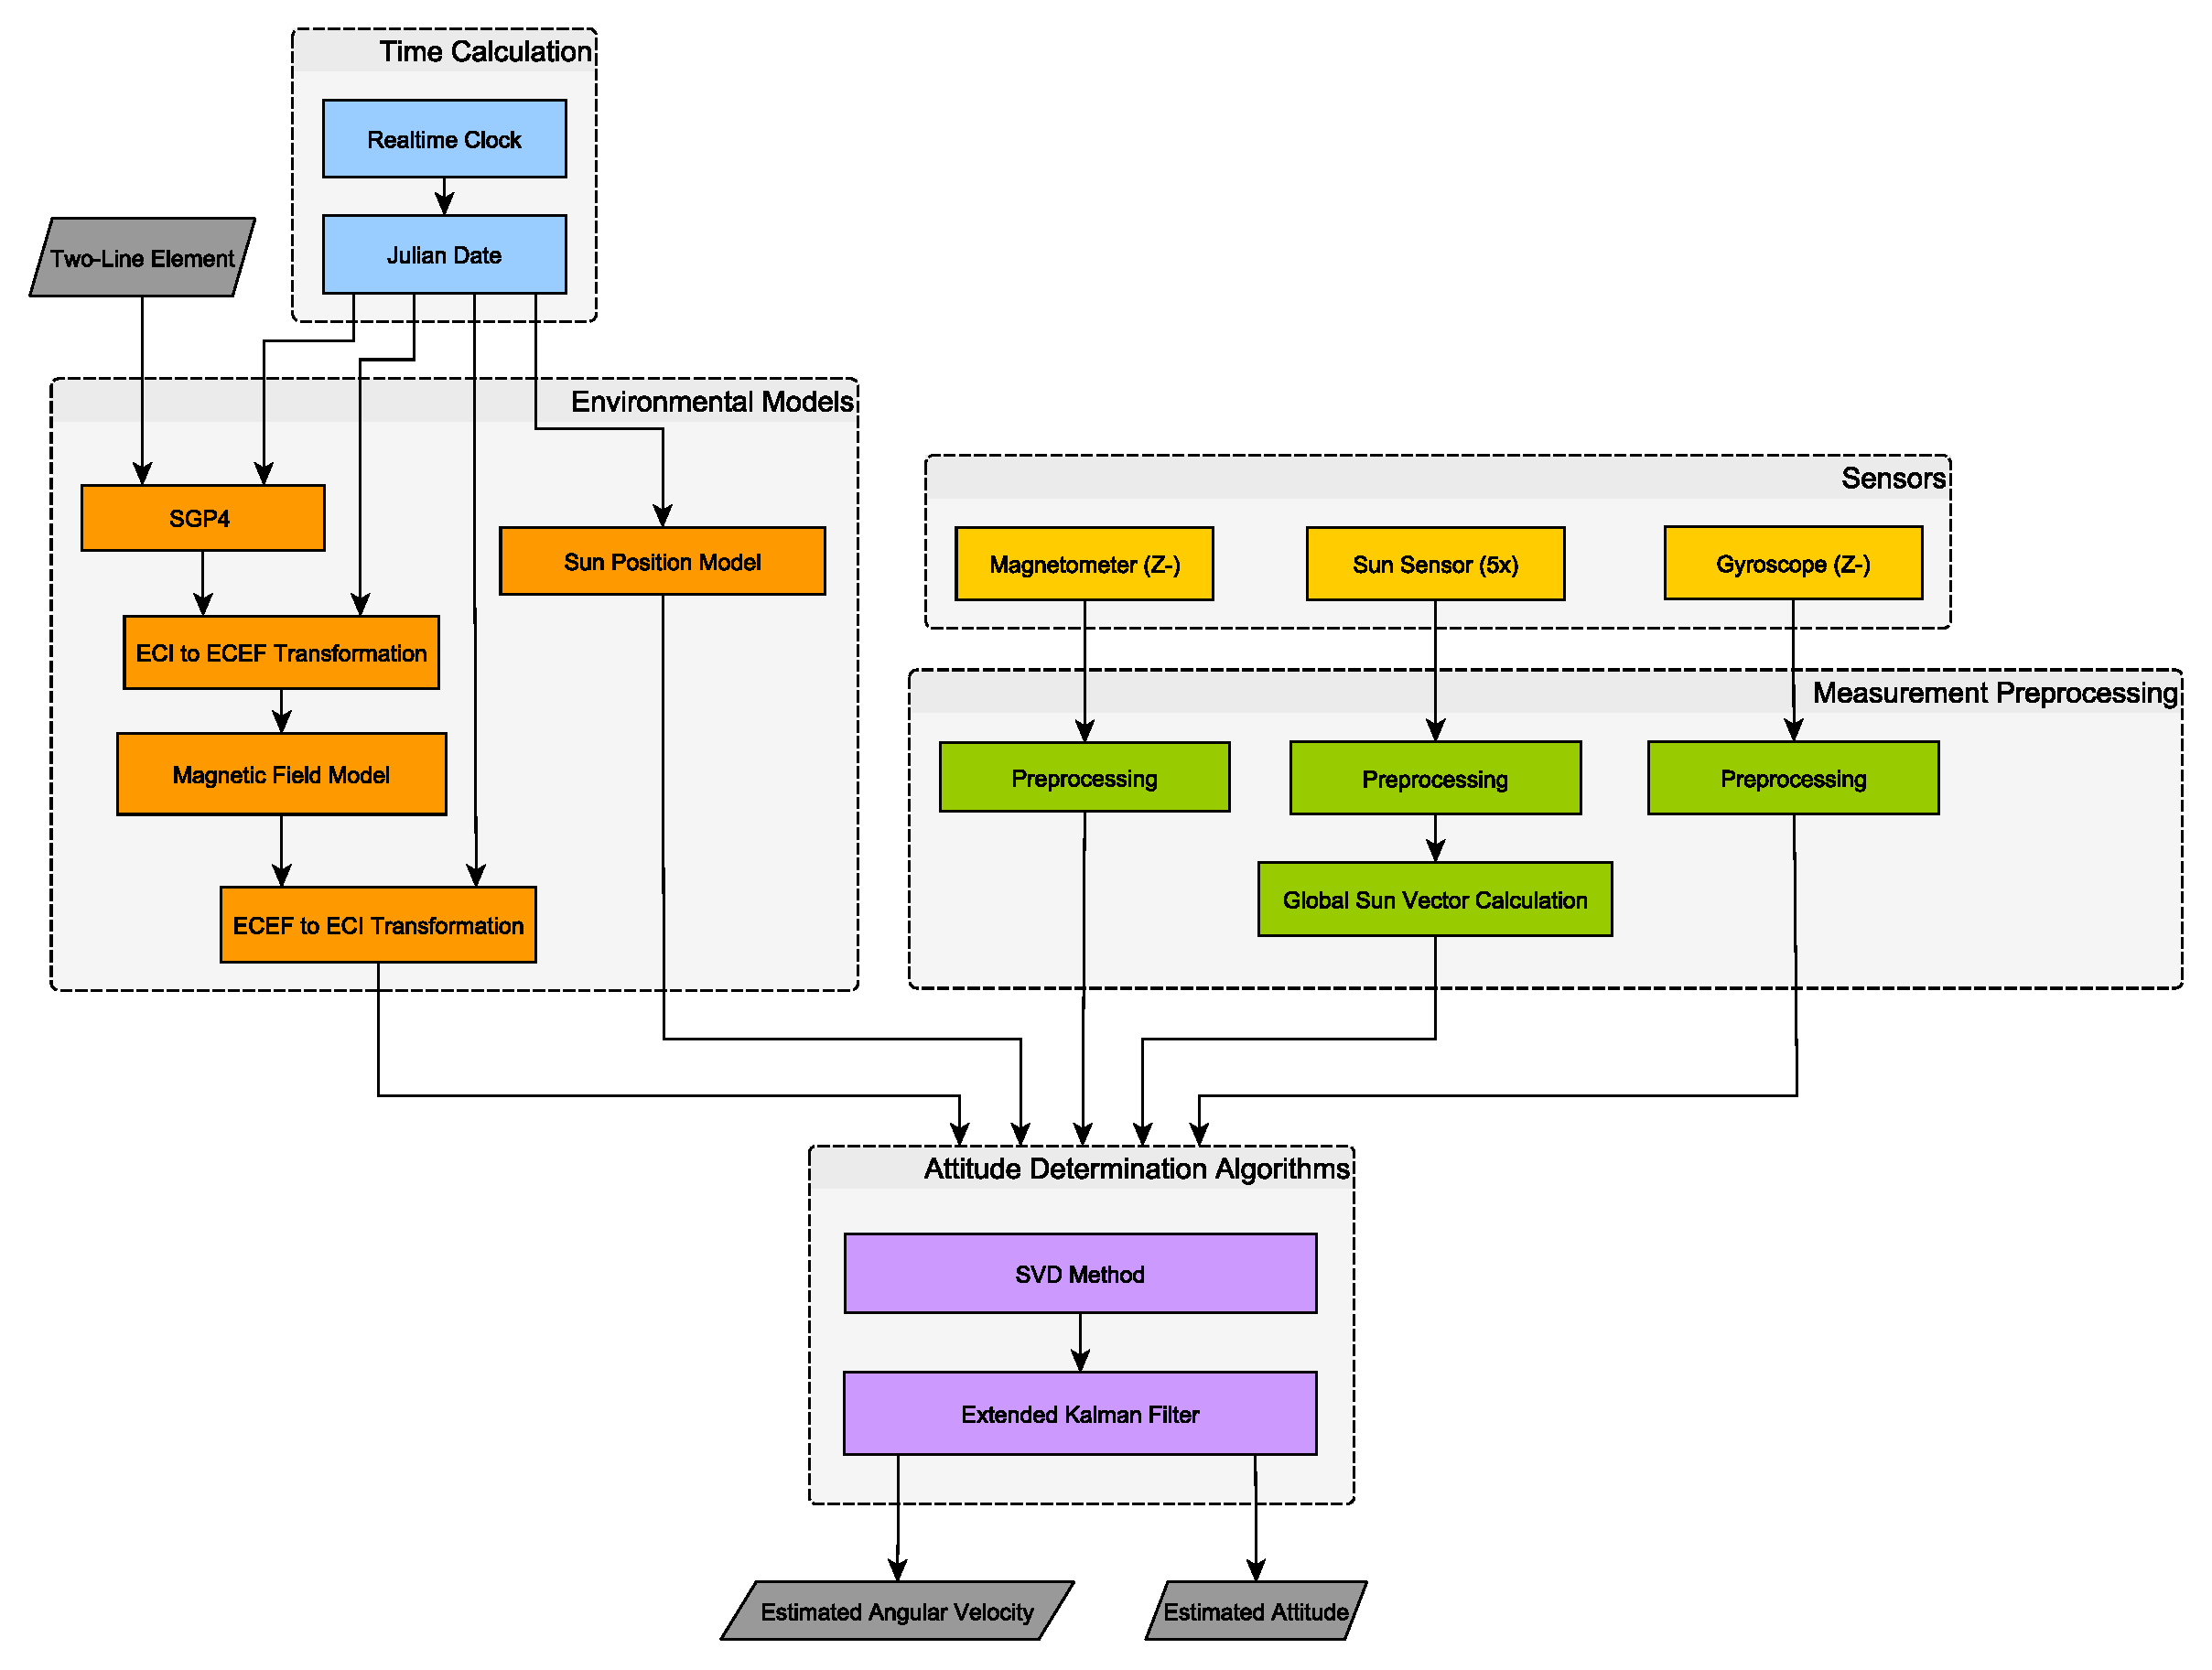
\includegraphics[width=0.5\columnwidth]{./Pictures/ATTDET_Architecture_new}
	\caption{Overview of the submodules that make up the complete Attitude Determination Systems from \cite{DavidThesis}}
	\label{fig:ADS_overview}
\end{figure}            

\subsection{Models Used in Attitude Determination}\label{subsec:ModelADS}
There are two main models used in the ADS. It is sun position model and a model of the earth's magnetic field. The output from both of this models are normalized vectors resolved in the ECI frame. The vectors will be used as reference vectors in both the SVD and the EKF. 

The sun model is the one described in \cite{AstroPC}. The sun model requires the Julian Date. The Julian Data is calculated from the real time clock that is part of the ADCS. The clock can also be resynchronized to the system time of the satellite \cite{DavidThesis}. 

The model of the earth's magnetic filed is the International Geomagnetic Reference Model (IGRF)\cite{IGRF}. The IGRF needs the orbit position as an input. To get the orbit the Simplified General Perturbation Model 4 (SGP4) is used, it is described in more detail in \cite{SGM4}. This model requires a Two Line Element (TLE) and the Julian Data to function. The IGRF needs the position of the satellite in Earth Centered Earth Fixed (ECEF) frame and to outputs the magnetic field vector in ECEF frame. Where ECEF is defined as origin at earth's center of mass. Z-axis aligned with the north pole, x-axis pointing towards the intersection between Earth's primary meridian and equator and the y-axis is defined to complete the coordinate frame according to the right hand rule. To accommodate this change in coordinates a function to generate the rotation matrix to go from ECI to ECEF frame was needed. This function is time dependent as the ECEF frame rotates in the ECI frame. The implementation of the SGI4, the IGRF and the function to find the rotation from ECI to ECEF frame are all based on the work in \cite{aausatMasterThisis} as stated by \cite{DavidThesis}. 

\subsection{SVD-Method to Solve Wahba's problem}
Wahba's problem is the least square optimization problem where you have a to minimize the cost function $J(A)$ show in \autoref{eq:Wahba'sProblem}. Where $b_i$ and $r_i$ are the same observations redissolved in two different frames. $A$ is an orthogonal matrix representing the rotation from the frame of $r_i$ to $b_i$ \cite{aausat}. So if $b_i$ are the observations from the models in ECI and $r_i$ are the sensor measurements in the body-fixed frame then by solving Wahba's problem you will get the rotation matrix from body-fixed frame to ECI.     

\begin{equation}\label{eq:Wahba'sProblem}
	J(A) = \sum\limits_{i=1}^{m}a_i||b_i - Ar_i||^2
\end{equation}

The cost function can be reformulated to \autoref{eq:Wahba'sProblemReformul} \cite{aausat}. Where $B = \sum\limits_{i=1}^{m}a_ib_ir_i^T$. It is clear now that this reduces Wahba's problem to maximizing $trace(AB^T)$, where the SVD-method is a fast and robust algorithm to solve this problem. For a more rigorous deduction of the algorithm see \cite{DavidThesis} or \cite{aausat}.

\begin{equation}\label{eq:Wahba'sProblemReformul}
	J(A) = \sum\limits_{i=1}^{m}a_i - trace(AB^T)
\end{equation}

\subsection{Extended Kalman Filter on MOVE-II}\label{chap:EKF_MOVE_II}
The full EKF will not be fully explained or derived in this report. Instead the key features and implementations will be highlighted. For a more in depth view into EKF see \cite{DavidThesis} or \cite{indirectKalman} which is the derivation followed here.  

The EKF that is used on the MOVE-II satellite is not based on the dynamic model of the satellite, but rather uses the gyroscope measurements directly in the models. Rather than using it as a measurement. This means that the gyroscope measurements replaces the dynamic model. This has two main advantages. The first is that the gyroscope measurements might be more accurate than the dynamic model. The second is that this method is a lot less computational expensive. To use the gyroscope measurements to replace dynamic model a model of the gyroscopes is instead needed. The gyroscope can be modeled as shown in \autoref{eq:gyroModel}. Where $\tilde{\boldsymbol{\omega}} \in \mathbb{R}^{3}$ is the measured angular velocity from the gyroscope and $\boldsymbol{\omega} \in \mathbb{R}^{3}$ is the true angular velocity. $\boldsymbol{\beta} \in \mathbb{R}^{3}$ is the bias of the gyroscope modeled as a random walk. $\boldsymbol{\eta_v} \in \mathbb{R}^{3}$ and $\boldsymbol{\eta_u} \in \mathbb{R}^{3}$ are independent Gaussian with white noise with zero mean.               

\begin{align}
	\tilde{\boldsymbol{\omega}} &= \boldsymbol{\omega} + \boldsymbol{\beta} + \boldsymbol{\eta_v}\label{eq:gyroModel}\\
	\dot{\boldsymbol{\beta}} &= \boldsymbol{\eta_u}\label{eq:randomWalk} 
\end{align}

The state vector for the EKF is defined as $\boldsymbol{x} \in \mathbb{R}^{7}$ consisting of the rotation quaternion representing the rotation between body-fixed frame and ECI frame $q \in \mathbb{R}^{4}$ and the gyroscope bias $\boldsymbol{\beta} \in \mathbb{R}^{3}$.

\begin{equation}\label{eq:stateVectorEKF}
	\boldsymbol{x} = \begin{bmatrix}
    		\boldsymbol{q} \\ \boldsymbol{\beta} & 
		 \end{bmatrix}\\
\end{equation}

Given the gyroscopic \autoref{eq:gyroModel} a system of differential equation for the states can be written as \autoref{eq:diffEq}  
\begin{subequations}\label{eq:diffEq}
\begin{align}
	\boldsymbol{\dot{q}} &= \frac{1}{2}\boldsymbol{\Omega}(\tilde{\boldsymbol{\omega}} - \boldsymbol{\beta} - \boldsymbol{\eta_v})\boldsymbol{q}\label{eq:diffQuaternion}\\
	\boldsymbol{\dot{\beta}} &= \boldsymbol{\eta_u}
\end{align} 
\end{subequations}

Where $\boldsymbol{\Omega}$ is defined in \autoref{eq:omega} and $[\cdot\times]$ is defined as skew-symmetric operation. 

\begin{equation}\label{eq:omega}
	\boldsymbol{\Omega}(\boldsymbol{\omega}) = \begin{bmatrix}
		-[\boldsymbol{\omega}\times]^T & \boldsymbol{\omega} \\
		-\boldsymbol{\omega}^T & 0 \\ 
		\end{bmatrix}
\end{equation} 

This leads to the propagation equation shown in \autoref{eq:propagation} at time k. Where $\hat{\cdot}$ is an estimate, + means the corrected estimate and - is the output from the propagation step. 

\begin{subequations}\label{eq:propagation}
\begin{align}
	\hat{\boldsymbol{\beta}}^-_k &= \hat{\boldsymbol{\beta}}^+_{k-1} \\
	\hat{\boldsymbol{\omega}}^-_k &= \tilde{\boldsymbol{\omega}}_k-\hat{\boldsymbol{\beta}}^+_{k-1} \\
	\hat{\boldsymbol{q}}^-_k &= (\boldsymbol{I}_{4\times4} + \frac{\Delta t}{2}\boldsymbol{\Omega}(\hat{\boldsymbol{\omega}}^+_{k-1}))\hat{\boldsymbol{q}}^+_{k-1}
\end{align}
\end{subequations}

For the update step the measurement vector $\boldsymbol{z}_k \in \mathbb{R}^{6}$ is defined as in \autoref{eq:measurment}. Where $\tilde{\boldsymbol{b}}_k \in \mathbb{R}^{3}$ is the measured magnetic vector and $\tilde{\boldsymbol{s}} \in \mathbb{R}^{3}$ is the measured sun vector at time $k$. 

\begin{equation}\label{eq:measurment}
	\boldsymbol{z}_k = \begin{bmatrix}
		\tilde{\boldsymbol{b}}_k \\
		\tilde{\boldsymbol{s}}_k \\
	\end{bmatrix}
\end{equation}  

The estimated measurement vector $\boldsymbol{h}_k \in \mathbb{R}^{6}$ is defined as in \autoref{eq:estimatedMeasurment}. Where $\boldsymbol{A}(\hat{\boldsymbol{q}}^-_k)$ is the rotation matrix from ECI frame to body-fixed frame based on the current uncorrected estimate of the quaternion $\hat{\boldsymbol{q}}^-_k$. $\boldsymbol{r}_{mag} \in \mathbb{R}^{3}$ is the reference vector for the magnetic field based on the IGRF model and $\boldsymbol{r}_{sun} \in \mathbb{R}^{3}$ is the reference vector from the sun position model. This means that $\boldsymbol{h}_k$ is the reference vectors resolved in the body-fixed frame.   

\begin{equation}\label{eq:estimatedMeasurment}
	\boldsymbol{h}_k = \begin{bmatrix}
		\boldsymbol{A}(\hat{\boldsymbol{q}}^-_k)\boldsymbol{r}_{mag} \\
		\boldsymbol{A}(\hat{\boldsymbol{q}}^-_k)\boldsymbol{r}_{sun} \\
	\end{bmatrix}
\end{equation}

The error vector $\boldsymbol{\epsilon}_k \in \mathbb{R}^{6}$ is then defined as the difference between the measurement vector $\boldsymbol{z}_k$ and the estimated measurement vector $\boldsymbol{h}_k$, as shown in \autoref{eq:errorVector}. 

\begin{equation}\label{eq:errorVector}
	\boldsymbol{\epsilon}_k = \boldsymbol{z}_k - \boldsymbol{h}_k
\end{equation}  

For the correction step the estimate of the error state vector $\delta\hat{\boldsymbol{x}}_k \in \mathbb{R}^{6}$ shown in \autoref{eq:errorStateVector}.       

\begin{equation}\label{eq:errorStateVector}
	\delta\hat{\boldsymbol{x}}_k = \begin{bmatrix}
		\delta\hat{\boldsymbol{\vartheta}}_k \\
		\delta\hat{\boldsymbol{\beta}}_k \\
	\end{bmatrix}
\end{equation} 

Where the relations between $\delta\hat{\boldsymbol{\vartheta}}_k$ and $\delta\hat{\boldsymbol{q}}^+_k$ is shown in \autoref{eq:stateRelation}.

\begin{equation}\label{eq:stateRelation}
	\delta\hat{\boldsymbol{q}}^+_k = \frac{1}{\sqrt{1- ||\delta\hat{\boldsymbol{\vartheta}}_k||^2/4}}\begin{bmatrix}
			\delta\hat{\boldsymbol{\vartheta}}_k/2 \\
			1 \\
		\end{bmatrix}
\end{equation}

$\delta\hat{\boldsymbol{q}}^+_k$ represent the error between the true quaternion and the estimated one. It is represented as the rotation between the true quaternion and the estimated quaternion instead of as a simple arithmetic as this leads to numerical issues \cite{DavidThesis}. It is defined by \autoref{eq:errorQuaternion}. $\delta\hat{\boldsymbol{\beta}}_k$ is simply defined as the difference between the true bias and the estimated bias as shown in \autoref{eq:errorBias}.

\begin{subequations}
\begin{align}
	\boldsymbol{q} &= \delta\boldsymbol{q}\otimes\hat{\boldsymbol{q}}\label{eq:errorQuaternion} \\
	\delta\boldsymbol{\beta} &= \boldsymbol{\beta} - \hat{\boldsymbol{\beta}}\label{eq:errorBias} 
\end{align}
\end{subequations} 

The error state vector $\delta\hat{\boldsymbol{x}}_k$ is calculated by \autoref{eq:calcErrorState}. Where $\boldsymbol{K}$ is the Kalman gain. 

\begin{equation}\label{eq:calcErrorState}
	\delta\hat{\boldsymbol{x}}_k = \boldsymbol{K}\boldsymbol{\epsilon}_k
\end{equation}

This finely leads to the correction step show in \autoref{eq:correctionStep}. 

\begin{subequations}\label{eq:correctionStep}
\begin{align}
	\hat{\boldsymbol{q}}^+_k &= \delta\hat{\boldsymbol{q}}^+_k\otimes\hat{\boldsymbol{q}}^-_k \\
	\hat{\boldsymbol{\beta}} &= \hat{\boldsymbol{\beta}}^-_k + \delta\hat{\boldsymbol{\beta}}^+_k 
\end{align}
\end{subequations} 

